
\chapter{Permian Basin Background}
\label{CHAP:3}



%1. Oil and gas production from horizontal drilling and fracking
%2. Induced seismicity: historical in Texas
%3.  Why is it happening?
  % Basic mechannisms of induced. pore pressure, mohr circle
  % other methods to tie: spatio temporal linking. more plausible when there are many simultaneous factors
 % 4. recent stuff (figure from GRL)
 % Why hard to 

%1. different theories of causes 
%2. difficulty in the Delaware basin case due to density
%3. Difficulty of observing subsurface changes

Texas has been a leading producer of oil and gas for over a century \citep{Frohlich2016HistoricalReviewInduced, TheAcademyofMedicine2017EnvironmentalCommunityImpacts}. It became the nation's largest producer of crude oil after the first successful vertical well was drilled south of Beaumont, TX in 1901. These ``conventional'' wells were the primary mode of production in multiple oil fields across the state. It wasn't until the early 2000s that advances horizontal drilling and hydraulic fracturing (also known as fracking, Figure \ref{fig:oil-drilling}) opened up vast new shale resources which were previously unworkable \citep{Waters2006Spe103202Ms}. 
For example, the Wolfcamp shale in Texas' Permian Basin is the largest continuous oil field that has ever been discovered in the United States, containing 20 billion barrels of oil and 16 trillion cubic feet of gas \citep{Gaswirth2016AssessmentUndiscoveredContinuous}. While areas of the Wolfcamp shale in the Midland Basin have been traditionally developed using vertical wells, the ability to extend subsurface drilling horizontally (Figure \ref{fig:oil-drilling}b) and increase production using enhanced oil recovery (EOR, Figure \ref{fig:oil-drilling}d)
allowed many new areas to be economically viable for oil and gas production.

%Figure \ref{fig:oil-drilling} shows a simplified diagram of the operation techniques of horizontal drilling, hydraulic fracturing, wastewater disposal, and enhanced oil recovery.
%These shale resources are also known as ``tight oil` and ``shale gas'', and may collectively be referred to as ``unconventional''. 


\begin{figure}
	\centering
%	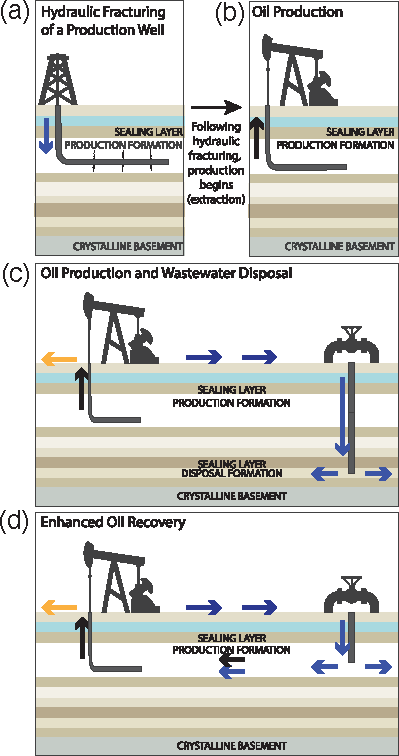
\includegraphics[width=0.6\linewidth]{figures/chapter3-permian/oil-page.pdf}
	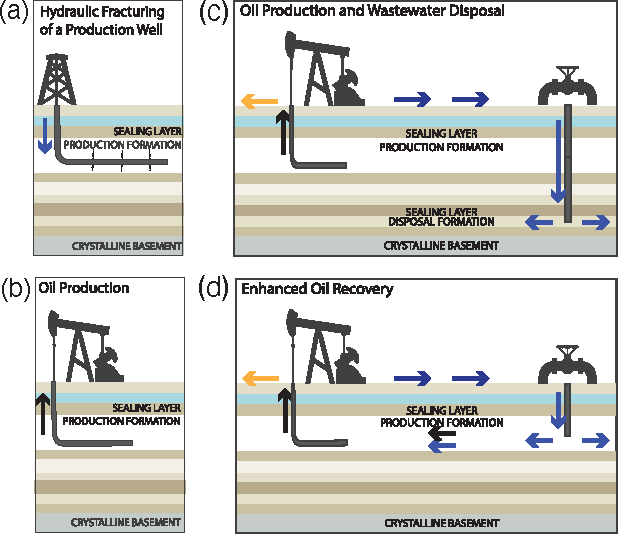
\includegraphics[width=\linewidth]{figures/chapter3-permian/oil-page-square.pdf}
	\caption[Diagram of unconventional oil production operations]{
		Simplified diagrams of oil-field operations. Arrows show the directions of fluid being injected or withdrawn. Arrow color indicates the contents of the fluid: black (oil, gas, and wastewater), yellow (oil and gas), and blue (wastewater). 
		(a) In a hydraulic fracturing operation, fluids are injected at high pressure into a production well, causing fractures in the surrounding rock that increase permeability. Increased permeability allows the extraction of oil or gas from a larger region. Following the hydraulic fracturing of a well, the well goes into production (b). 
		(c) Production wells extract oil and gas, and as a byproduct, salt water (commonly called ``produced water'' or ``wastewater''), which is injected to a different subsurface formation at a disposal well. 
		(d) Enhanced oil recovery (EOR), an alternative to wastewater disposal, involves injecting the water back into the formation holding the oil and gas to sweep oil and gas toward the production well.
		(Figure adapted from \citep{Rubinstein2015MythsFactsWastewater})
	}
	\label{fig:oil-drilling}
\end{figure}

%This report uses the term “shale” to describe organic rich formations containing natural gas (shale gas) and/or oil (tight oil) that require multiple hydraulic fractures, usually created from long wells drilled horizontally, to produce hydrocarbons profitablyThe term “tight oil” may include hybrid formations containing oil that has migrated into very tight rock. Many experts refer to shale gas and tight oil resources collectively as “unconventional.” \cite{TheAcademyofMedicine2017EnvironmentalCommunityImpacts}
%lthough these resources have been known to exist for decades, rapid expansion of oil and gas production from shale formations was made possible by the innovative combined use of two technologies—hydraulic fracturing (referred to colloquially as “fracking”) and horizontal drilling.



Despite the economic benefits that the new production technologies provided for Texas, concerns have been raised about possible environmental consequences to shale development \citep{TheAcademyofMedicine2017EnvironmentalCommunityImpacts, Scanlon2020WillWaterIssues}. 
%including injection of chemicals underground, water usage in semiarid areas and potential water contamination, and seismic activity
%For example, more than 30 billion bbl of wastewater have been disposed throughout the Permian Basin \cite{Lemons2019SpatiotemporalStratigraphicTrends} and future Wolfcamp shale development is expected to generate $\sim$300 billion bbl of produced water \cite{Smye2021VariationsVerticalStress,  Scanlon2020WillWaterIssues}.
%Here we briefly review the  seismic activity induced from oil and gas production.
One concern is the triggering of seismic activity, as it has been recognized that injection or withdrawal of fluids from the subsurface can induce earthquakes along existing faults \citep{Ellsworth2013InjectionInducedEarthquakes, Simpson1988TwoTypesReservoir}.
Note that induced earthquakes are not limited to oil and gas operations \citep{Grigoli2017CurrentChallengesMonitoring, Foulger2018GlobalReviewHuman, Baan2017HumanInducedSeismicity}; they have also been associated with geothermal energy development \citep{Deichmann2009EarthquakesInducedStimulation}, mining operations \citep{Hasegawa1989InducedSeismicityMines}, water impoundment in reservoirs \citep{Talwani1997NatureReservoirInduced}, and CO$_2$ sequestration \citep{Gan2013GasInjectionMay}.



%2. Induced seismicity: historical in Texas
%3.  Why is it happening?
% Basic mechannisms of induced. pore pressure, mohr circle
% other methods to tie: spatio temporal linking. more plausible when there are many simultaneous factors



% 
%During this time period, an increase in low magnitude earthquakes was observed. While West Texas had few seismic monitoring stations set up, one array near Lajitas, TX had been operating since 2000 \citep{Frohlich2019OnsetCauseIncreased}.


\begin{figure}
	\centering
	%	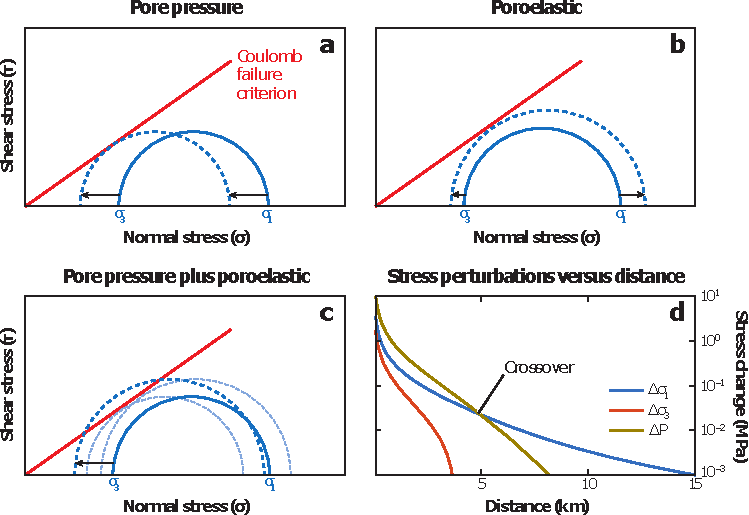
\includegraphics[width=\linewidth]{figures/chapter3-permian/mohr-circles.pdf}
	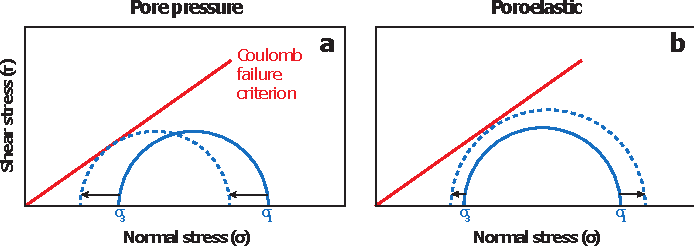
\includegraphics[width=\linewidth]{figures/chapter3-permian/mohr-circles-toponly.pdf}
	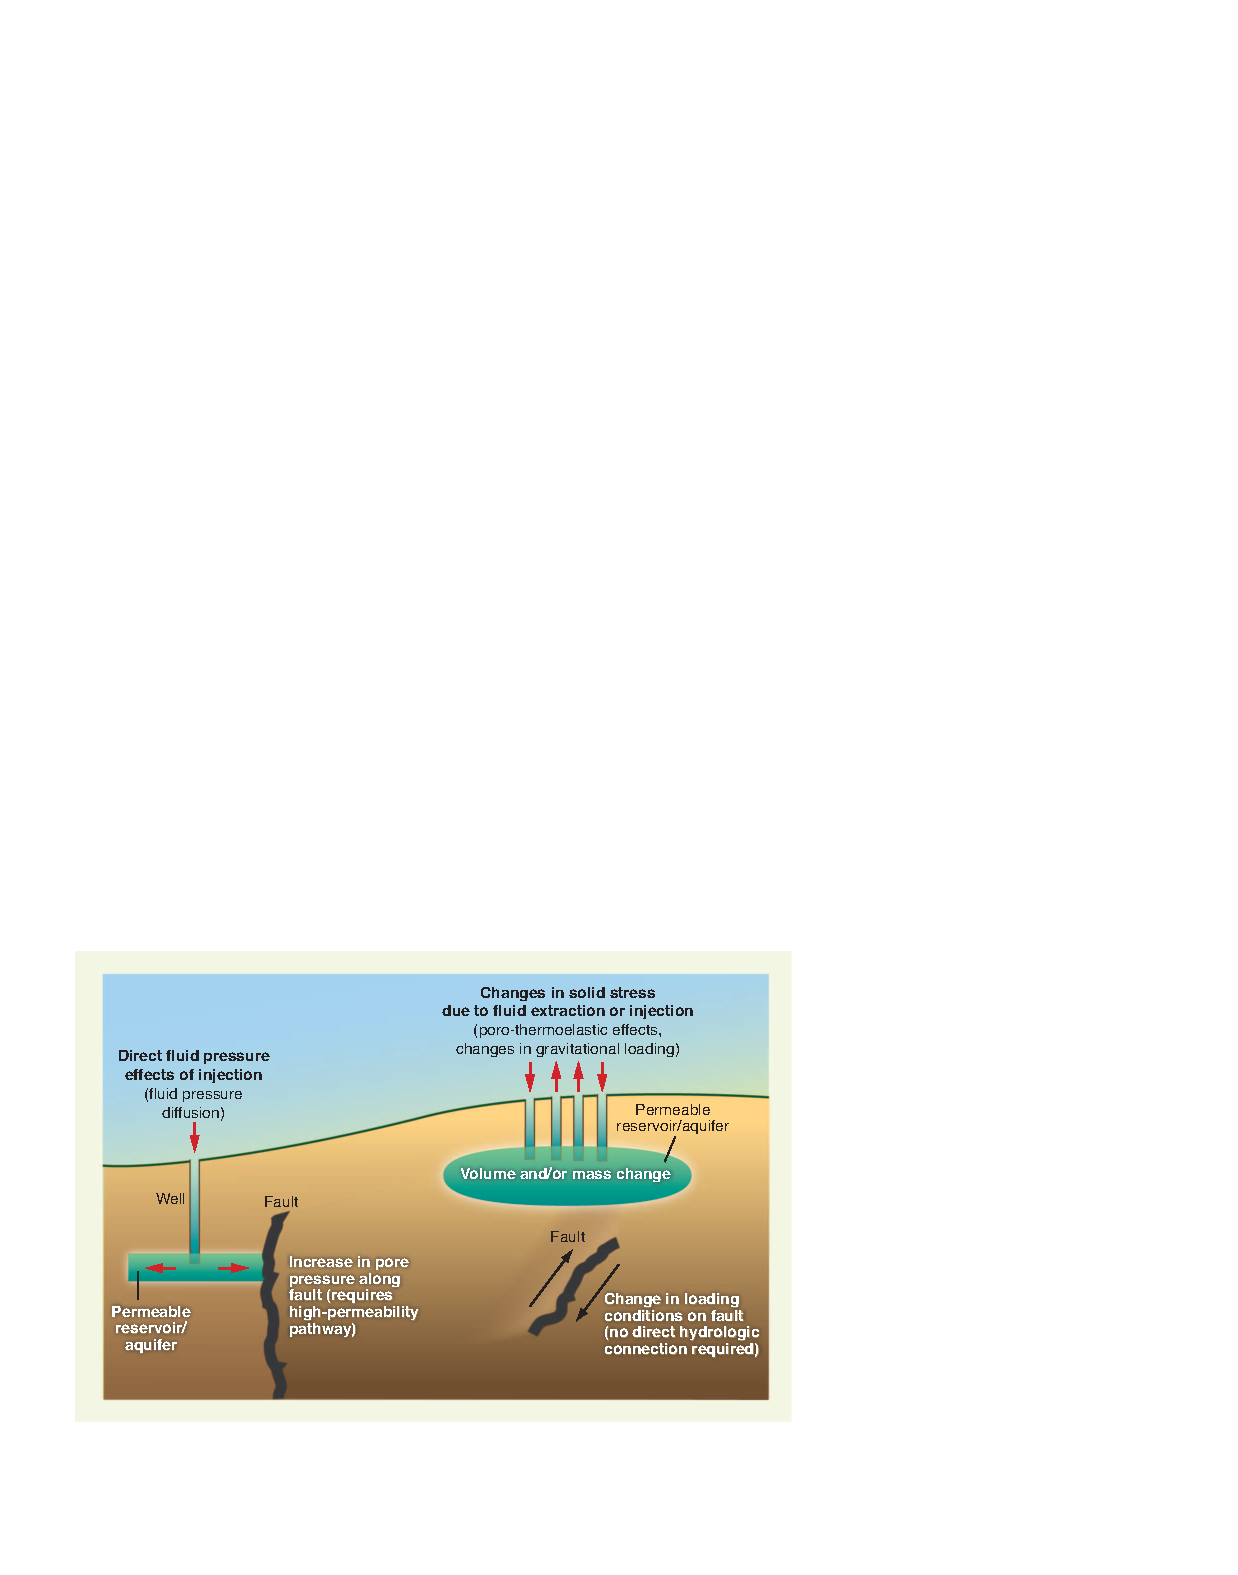
\includegraphics[width=\linewidth]{figures/chapter3-permian/injection-ellsworth.pdf}
	\caption[Effects of pore pressure perturbations and poroelastic stress changes on fault failure]{
		Effects of pore pressure perturbations and poroelastic stress changes on fault failure. Solid curves represent the initial stress state, and dashed curves represent the perturbed stress state. (a) Increased pore pressure reduces normal stress on the fault plane, moving the fault closer to the Coulomb failure criterion. (b) Poroelastic stresses increase differential stress. For both (a) and (b), pore pressure perturbations and stress changes, as well as the relative magnitude of changes, depend on parameters including time, distance, injection rate, diffusivity, and poroelastic parameters.
		(Bottom) Schematic diagram for each mechanism causing injection-induced earthquakes.
		(Top from \cite{Keranen2018InducedSeismicity}, bottom from \cite{Ellsworth2013InjectionInducedEarthquakes})
	}
	\label{fig:mohr-circles}
\end{figure}

One conceptual model for triggering earthquakes uses the Mohr-Coulomb failure criterion \citep{Hubbert1959RoleFluidPressure}.
The critical shear stress $\tau_{critical}$ required to promote fault slippage can be written as
\begin{equation}
\tau_{critical} = \tau_0 + \mu (\sigma_n - P)
\end{equation}
where $\tau_0$ is the cohesive strength of the sliding surface (often negligible), $\mu$ is the coefficient of friction, $\sigma_n$ is the normal stress, $P$ is the pore pressure \citep{Nicholson1990EarthquakeHazardAssociated, Ellsworth2013InjectionInducedEarthquakes}. Intuitively, increasing the shear stress or decreasing the normal stress ``unclamps'' the fault and encourages failure \citep{Shearer2019IntroductionSeismology}. Since increasing pore pressure lowers the effective normal stress, fluid injection can move critically stressed faults to failure and cause earthquakes (Figure \ref{fig:mohr-circles}a).
Alternatively, poroelastic effects from injection can change the loading conditions on a fault without a direct hydraulic connection, which can cause fault failure through increased differential stress (Figure \ref{fig:mohr-circles}b).

%This was determined to be the cause of many earthquakes in Oklahoma in 2014-2016 (cite). However, other causes may play a role in the Permian Basin earthquakes, including poroelastic effects that may be a factor 10s of kilometers away from injection, even without direct hydraulic connections \citep{Skoumal2020InducedSeismicityDelaware}


%Pressure from wastewater injection may play a role in certain areas (find that citation). This increasing of subsurface pore pressure could cause surface uplift in certain cases, and an example of this was reported on a single injection well (and single CO2 injection?) by \cite{Kim2018AssociationLocalizedGeohazards}.s



%Following \cite{Dahm2012RecommendationDiscriminationHuman}, we can classify these discrimination methodsin three main families: physics-based methods, statistics-based methods, and source parameters-basedmethods




In Texas, earthquakes have occurred in close association with petroleum activities since 1925, but the rate of earthquakes in the last decade has increased over tenfold \citep{Frohlich2016HistoricalReviewInduced, Skoumal2020InducedSeismicityDelaware}.
To better understand the causes of these earthquakes and to assess the likelihood of infrastructure damage and safety concerns, 
the State of Texas funded the Texas Seismological Network (TexNet) to record earthquakes down to M2.0 across the state since 2017 \citep{Savvaidis2019TexnetStatewideSeismological}. 
By that time, there were over 130,000 active production wells, 23,000 active EOR wells, and nearly 3800 active saltwater disposal (SWD) wells in the Permian Basin (Figure \ref{fig:permian-oil-6panel} (a)).  
The volumes of petroleum production (Figure \ref{fig:permian-oil-6panel} (b, c)) and wastewater injection (Figure \ref{fig:permian-oil-6panel} (e, f)) have been rising in many locations; however, the recently cataloged earthquakes are spatially clustered (Figure \ref{fig:permian-oil-6panel} (c)). One significant cluster is near Pecos, TX in the Delaware Basin, which experienced over 2000 earthquakes in 2017 \citep{Frohlich2019OnsetCauseIncreased}. 
%Subsequent activity has increased considerably, and the region experienced more than 2000 earthquakes in 2017. 


%TexNet seismic data will be most meaningful when combined with knowledge of the subsurface \citep{Council2013InducedSeismicityPotential, TheAcademyofMedicine2017EnvironmentalCommunityImpacts}; however, measuring the subsurface at a basin-scale is both expensive and technically challenging.

\begin{figure}[hbt!]
	\centering
	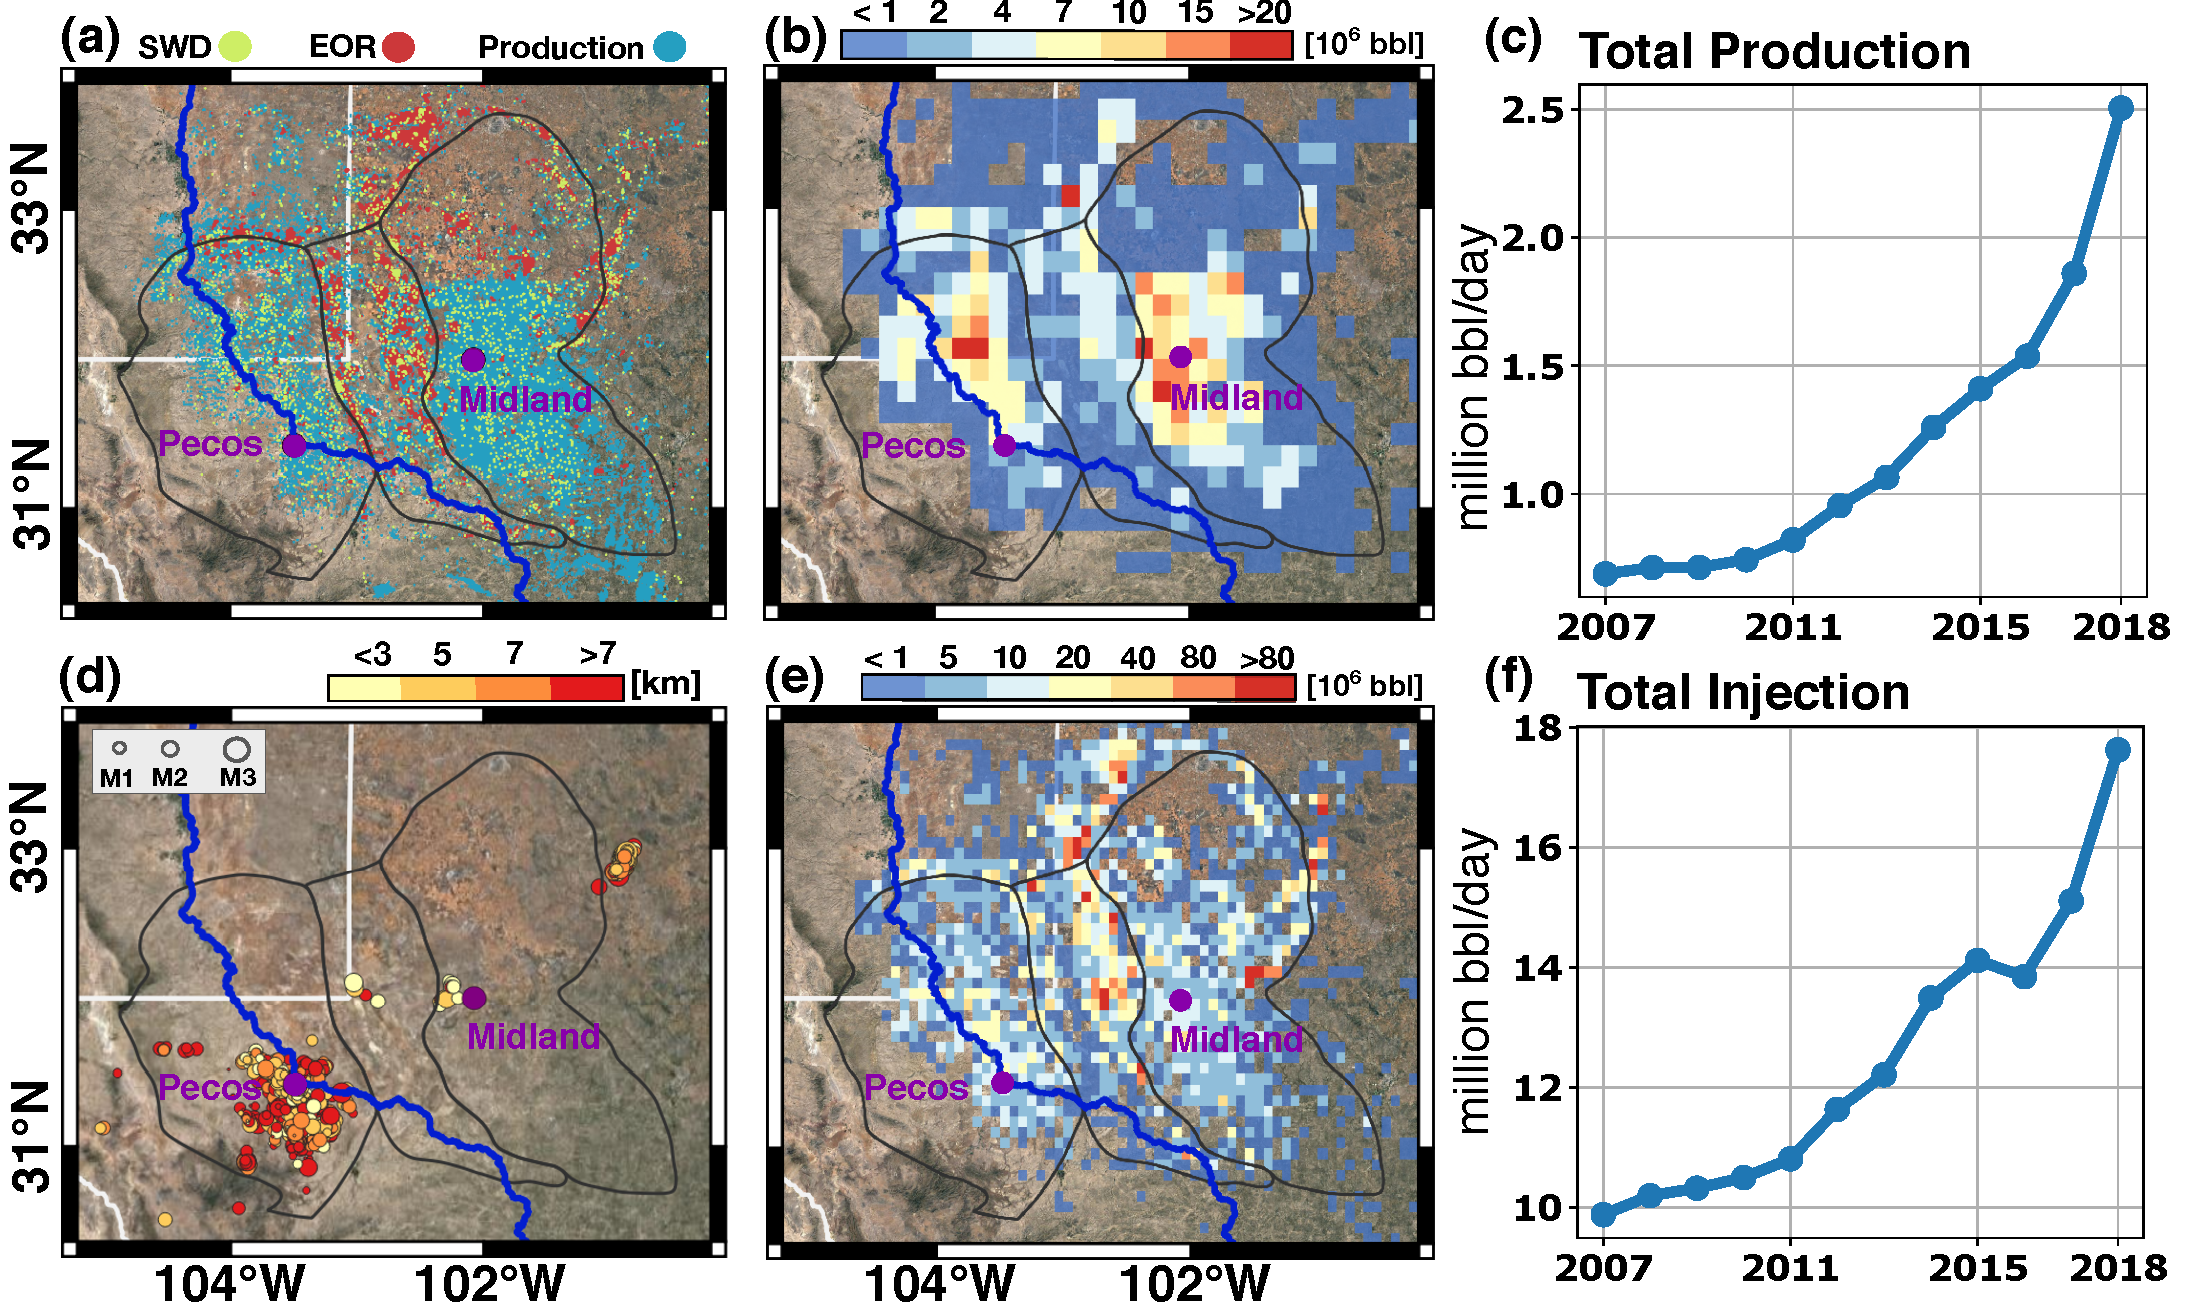
\includegraphics[width=0.99\linewidth]{paper1-permian/figures/supplement/figureS1-cisr-data.pdf}
	\caption[Shale development and seismicity in the Permian Basin.]{Shale development and seismicity in the Permian Basin through 2018. 
		(a) Locations of oil production, EOR, and saltwater disposal (SWD) wells active in 2017. (b) Annual oil production volume on a 10-mile grid in 2017. (c) Permian Basin oil production rate as reported by the Texas Railroad Commission. (d) Locations of earthquake hypocenters detected by TexNet in 2017. The color and size of a circle indicates the estimated earthquake depth and magnitude. (e) Annual injection volume (including both SWD and EOR wells) on a 5-mile grid. (f) Permian region injection rate (including both SWD and EOR wells) as reported by the Texas Railroad Commission.
	}
	\label{fig:permian-oil-6panel}
\end{figure}






%
%%\begin{figure}[hbt!]
%\begin{figure}
%	\centering
%	%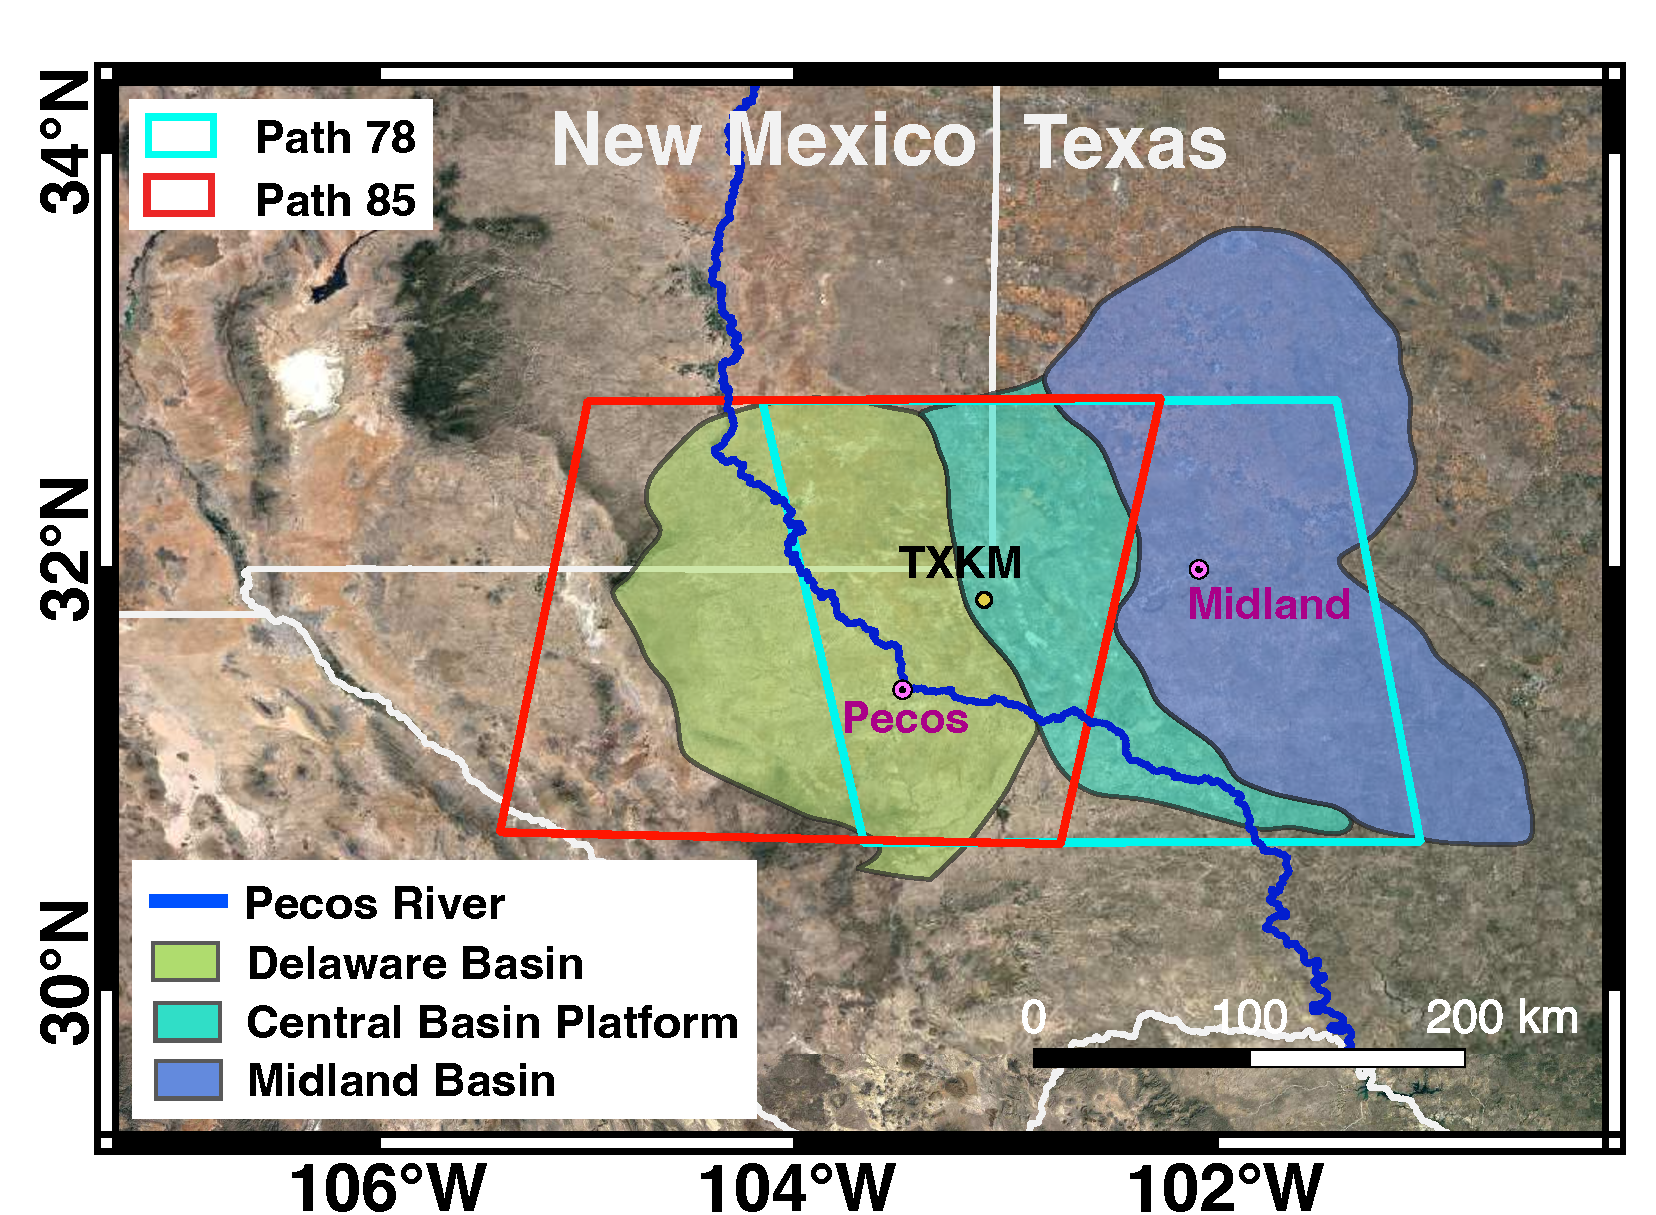
\includegraphics[width=0.9\linewidth]{figures/figure4-study-area.pdf}
%	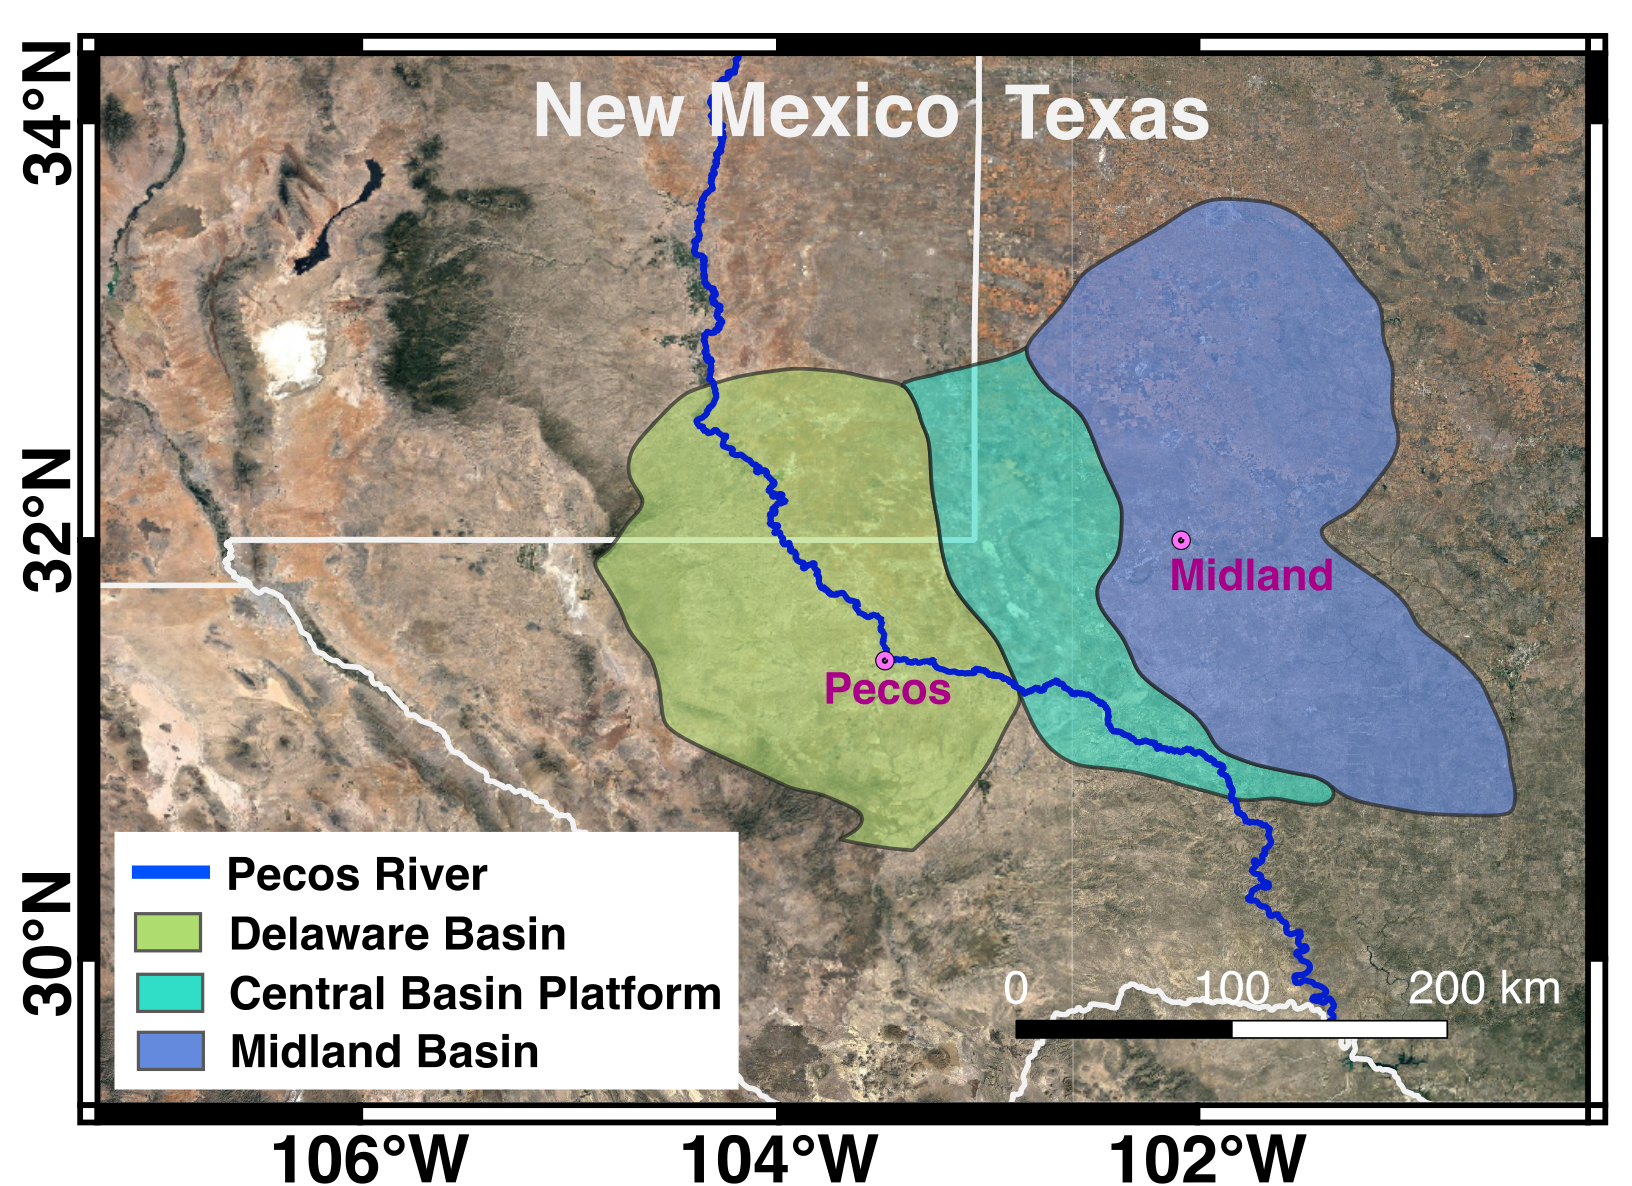
\includegraphics[width=0.96\linewidth]{figures/chapter3-permian/figure-study-area.png}
%	\caption[Subbasins within the Permian Basin]{
%		The subbasins of the Permian Basin are the Delaware Basin to the west (green) and Midland Basin to the east (purple), which are separated by the uplifed Central Basin Platform (teal).
%	}
%	\label{fig:study-area-plain}
%\end{figure}
%


% Intuitively, the spatial and temporal correlation between human activity and event occurrence may represent a key parameter to discriminate between natural and anthropogenic seismicity, but unfortunately this isnot always the case. Indeed, many industrial operations involving subsurface fluid injection (e.g., wastewaterdisposal) can transmit pore pressure changes at large distance, causing earthquakes several kilometers awayfrom the industrial site.


%Attributing causation of earthquakes to individual wells may be impossible in many cases due to the proximity of many wells, but 

Several studies have used spatio-temporal analyses to link certain instances of wastewater injection and hydraulic fracturing to earthquakes \citep{Savvaidis2020InducedSeismicityDelaware, Skoumal2020InducedSeismicityDelaware, Grigoratos2020EarthquakesInducedWastewatera}, but attributing causation of earthquakes to individual wells and discriminating induced from natural seismicity is extremely challenging \citep{Grigoli2017CurrentChallengesMonitoring, Dahm2012RecommendationDiscriminationHuman, Verdon2019ImprovedFrameworkDiscriminating,Frohlich2016HistoricalReviewInduced, Frohlich2016ReplyCommentA}.
%Without a detailed study involving multiple disciplines and observational datasets, 
%Recent efforts have considerably improved the public knowledge of subsurface fault locations (Horne?), geological characterization \citep{Smye2021LithologyReservoirProperties, Smye2021VariationsVerticalStress}, pore pressure distribution and... fault system stability \citep{Hennings2021StabilityFaultSystems} 
Understanding the nature and causes of earthquakes and how they are linked to certain production and disposal requires extensive knowledge of the subsurface.
However, subsurface measurements of pore pressure changes can be difficult or impossible to collect at a regional scale, and permanent GPS stations are too sparse to provide a full picture of surface changes.
InSAR surface deformation measurements provide a key observable, and they allow us to estimate locations of pressure build up from fluid injection, barriers to subsurface fluid flow, and unmapped faults. However, creating accurate maps of surface deformation using InSAR can be very challenging at the scale of the full Permian Basin.

In this thesis, we develop techniques for mitigating strong tropospheric noise to produce reliable surface deformation maps over large regions. These techniques are applicable to any large-scale deformation mapping, but they are critical to successfully detecting the centimeter-level changes occurring in the Permian Basin that are masked by 10s of centimeters of tropospheric noise. We begin in Chapter 3 by introducing the concepts required for mapping surface deformation over time using InSAR.




%Understanding the nature and causes of earthquakes and how they are linked to certain production and disposal wells requires extensive knowledge of the subsurface. InSAR surface deformation measurements allow us to estimate the distribution of fault slip at depth and infer the associated seismic risk \citep{Segall2010EarthquakeVolcanoDeformation, Huang2017FaultGeometryInversion}. Furthermore, measurements of reservoir inflation due to wastewater injection allows operators to assess pressure build-up in disposal aquifers and the associated triggered seismicity risk. It is also worth noting that oil recovery in shale wells is notoriously low \citep{Clark2009DeterminationRecoveryFactor}, and the performance of these wells varies significantly. InSAR can be employed to map subsurface fluid depletion and pressurization. These surface deformation observations, when coupled with reservoir compaction inversion modeling, can be used to assess the areal effectiveness of oil and gas extraction operations \citep{Du2001PoroelasticReservoirModel, Vasco2005UseQuasiStatic}. 


